\chapter{Importance Sampling}
There are two different ways to think about importance sampling.
The more traditional one is to go back to the primary problem that
Monte Carlo  wants to solve,
namely to approximate the value of an expectation
$\mu = \int \phi_0(x)dF_0(x) $ for some function $\phi_0$ and some CDF $F_0$.
However, $(\phi_0,F_0)$ is not the only pair $(\phi,F)$ for which
$\int \phi(x)dF(x) $ equals the specific number $\mu$. Indeed, given any other
CDF $F_1$,
\begin{align*}
	\mu & = \int \phi_0(x)dF_0(x)                      \\
	    & = \int \phi_0(x)\frac{dF_0}{dF_1}(x) dF_1(x) \\
	    & = \int \lambda(x)\phi_0(x)dF_1(x).
\end{align*}

where $\lambda(x)=\frac{dF_0}{dF_1}(x)$. If $F_0$, $F_1$ have densities
$f_0$, $f_1$, then $\lambda(x)=\frac{f_0(x)}{f_1(x)}$; if $F_0,$ $F_1$
have respective pmfs $f_0$, $f_1$, then also $\lambda(x)=\frac{f_0(x)}{f_1(x)}$
This raises the interesting possibility that we can sample from a general $F_1$, and
subsequently use the usual Monte Carlo estimate
\[
	\hat{\mu} = \frac{1}{n} \sum_{i = 0}^{n} \lambda(X_i)\phi_0(X_i) = E_{F_1}[\lambda(X_i)\phi_0(X_i)].
\]

where $X_1, X_2, \ldots, X_n$ is Monte Carlo sample from $F_1$.
Importance sampling poses the problem of finding an optimal choice of $F_1$ for which to sample,
so that $\hat{\mu}$ has the smallest possible variance.
The distribution $F_1$ hat ultimately gets
chosen is called the \textit{importance sampling distribution}.

We can visualize this method by an example.

\begin{example}
	Suppose we want to evaluate
	\[
		I = \int_{0}^{10} e^{-2 |x-5|} dx.
	\]
	doing it analytically we get $I = 0.9999$.

	Now, suppose $h(x) = e^{-2 |x-5|}$ then we want to evaluate
	\[
		I = \int_{0}^{10} h(x) dx
	\]
	Now,
	\begin{align*}
		\label{hx with U}
		I & = \int_{0}^{10} h(x) dx                                                                                                            \\
		  & = \int_{0}^{10} h(x)\frac{10}{10} dx                                                                                               \\
		  & = \int_{0}^{10} 10 \times h(x) \frac{1}{10} dx = \int_{0}^{10} 10h(x) p(x) dx \text{ where } p(x)\text{ pdf of }U(0,1) \numberthis \\
		  & = E_U[10 \times h(U)] \text{ where, }  U\sim U(0,10).
	\end{align*}

	By Ordinary Monte Carlo technique we can estimate $I$ by $\frac{1}{N}\sum_{i = 0}^{N} 10 \times h(U_i)$ where $U_i\sim U(0,10)$ for $i=1,2,\ldots,N$
	for the large number of $N$.
	\begin{figure}[H]
		\centering
		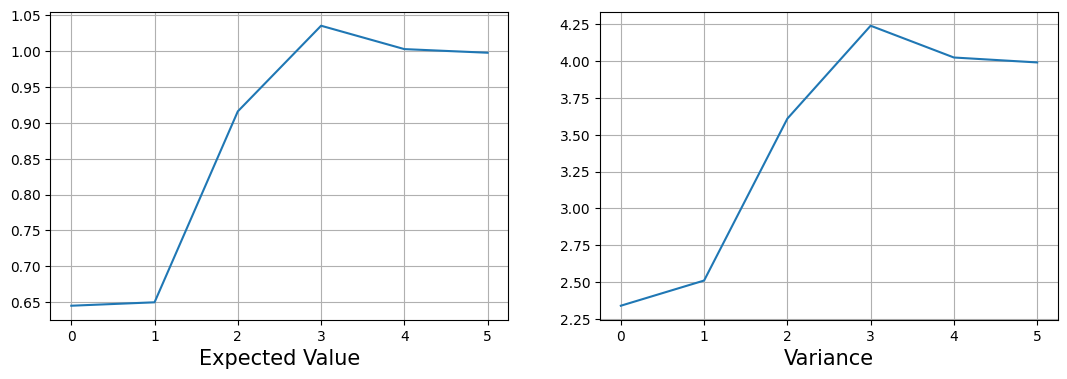
\includegraphics[width=0.8\textwidth]{int_h(x)_MC.png}
		\caption{Monte Carlo integration of $\int_{0}^{10} e^{-2 |x-5|} dx$.}
		\label{MC:IntegrationOFe-2|x*5|}
	\end{figure}
	\begin{table}[h]
		\centering
		\begin{tabular}{lcc}
			\hline
			Sample Size & Estimated Value I=0.9999 & Variance \\
			\hline
			10          & 2.3243                   & 5.6912   \\
			100         & 1.0372                   & 3.6717   \\
			1000        & 0.8871                   & 3.5543   \\
			10000       & 1.0467                   & 4.2416   \\
			100000      & 1.0053                   & 4.0089   \\
			1000000     & 1.0054                   & 4.0346   \\
			\hline
		\end{tabular}
		\caption{Monte Carlo integration of $\int_{0}^{10} e^{-2 |x-5|} dx$.}
		\label{tab:IntegrationOFe-2|x*5|}
	\end{table}
	Here we can see that for sample size 1M we get a pretty good estimation of $I$ with less then $0.6\%$ error but the variance is very high.
	If we see at left of Figure (\ref{fig:hxwithU01andN01}) we can see we are taking unnecessary value from low frequency part of $h(x)$ that is,
	from extream left and right. If we use choose an importance sampling distribution that has similar curve as $h(x)$ then we can estimate $I$ with low variance.
	If we choose importance sampling distribution as $N(5,1)$ then we see from right of Figure (\ref{fig:hxwithU01andN01}) it has similar pattern as $h(x)$.
	\begin{figure}[H]
		\centering
		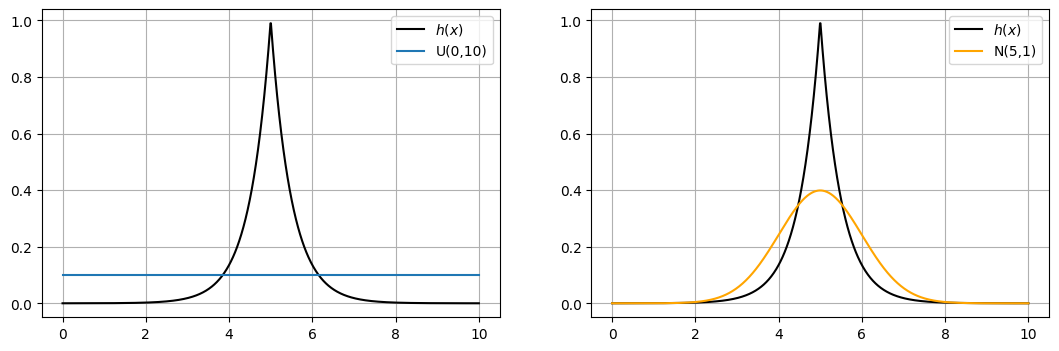
\includegraphics[width=0.8\textwidth]{h(x)_with_normal_and_uniform.png}
		\caption{$h(x)$ with $U(0,1)$ and $N(5,1)$}
		\label{fig:hxwithU01andN01}
	\end{figure}

	Let, $q(x)$ is pdf of $N(0,1)$ then, from (\ref{hx with U})
	\begin{align*}
		I & = \int_{0}^{10} 10h(x) p(x) dx                                            \\
		  & = \int_{0}^{10} 10 h(x) \frac{p(x)}{q(x)} q(x)dx                          \\
		  & = E_X\left[ 10 h(X) \frac{p(X)}{q(X)} \right] \text{ where } X\sim N(5,1) \\
		  & = E_X\left[ 10 h(X) \lambda(X) \right]\text{ where } X\sim N(5,1)
	\end{align*}
	Where, $\lambda(x) = \frac{p(X)}{q(X)}$ here $p(x)$ is pdf of $U(0,1)$ and $q(x)$ is pdf of $N(5,1)$. Now using usual Monte Carlo estimate
	\[
		I = \frac{1}{N} \sum_{i = 0}^{N} 10 h(X_i) \lambda(X_i)
	\]
	where $X_1, X_2,\ldots,X_N$ is Monte Carlo sample from $N(5,1)$.
	\begin{figure}[H]
		\centering
		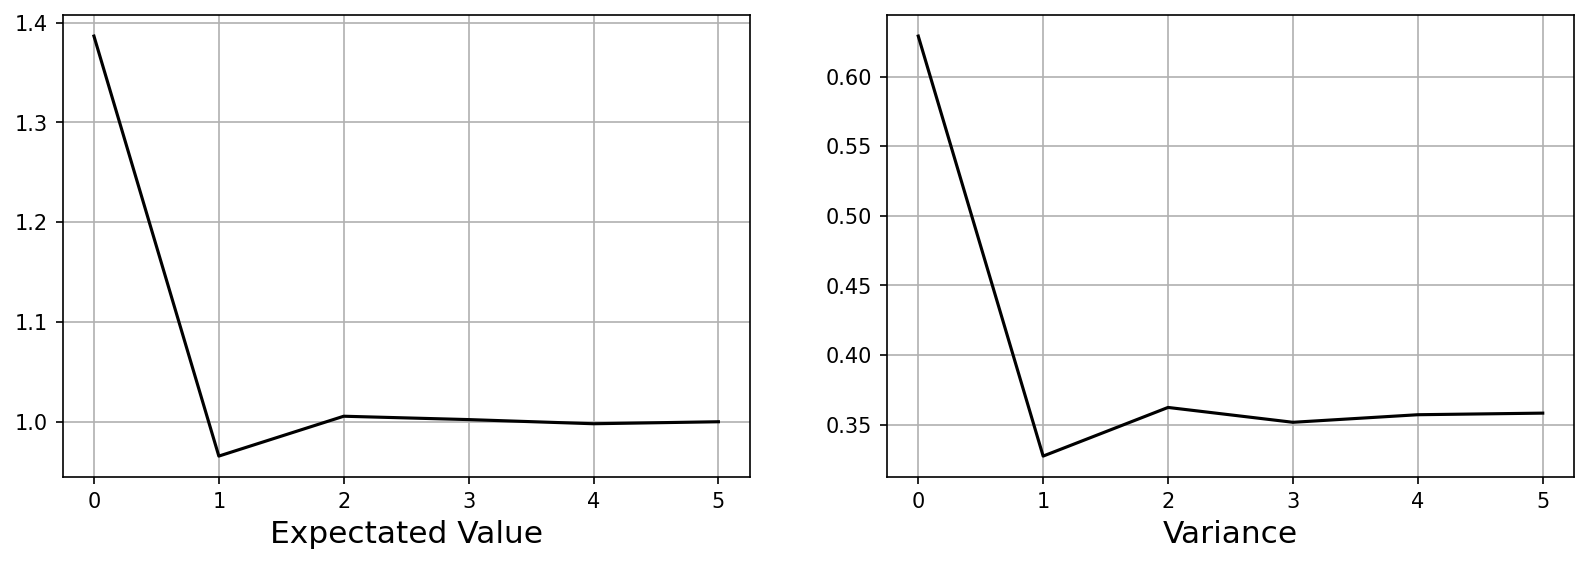
\includegraphics[width=0.8\textwidth]{int_h(x)_ipsam.png}
		\caption{Evaluating $\int_{0}^{10} e^{-2 |x-5|} dx$ using Importance Sampling.}
		\label{fig:impotrancesampling1}
	\end{figure}
	\begin{table}[h]
		\centering
		\begin{tabular}{lcc}
			\hline
			\textbf{Sample Size} & \textbf{Estimated Value (I=0.9999)} & \textbf{Variance} \\
			\hline
			10                   & 1.2473                              & 0.3812            \\
			100                  & 0.9292                              & 0.2593            \\
			1000                 & 1.0018                              & 0.3550            \\
			10000                & 1.0072                              & 0.3603            \\
			100000               & 1.0039                              & 0.3595            \\
			1000000              & 0.9999                              & 0.3580            \\
            \hline
		\end{tabular}
		\caption{Evaluating $\int_{0}^{10} e^{-2 |x-5|} dx$ using Importance Sampling.}
		\label{tab:mytable}
	\end{table}
\end{example}



A more contemporary view of importance sampling is that we do not approach
importance sampling as an optimization problem, but because the circumstances
force us to consider different sampling distributions $F$.

Now, we also assume that $F_0,$ $F_1$ both have densities, say $f_0$, $f_1$.
